\documentclass{beamer}

\begin{document}
	
	\begin{frame}
	\frametitle{Lines: General Idea}
		\begin{itemize}
			\item Find the number of lines on frame A, then on the next frame denoted as frame B, find the number of lines on it, too.
			
			\pause
			
			\item If the two frames have the same or similar number of lines, then there are probably no scene change in the time interval of the two frames.
			
			\pause
			
			\item How do we find lines?
		\end{itemize}
	\end{frame}
	
	\begin{frame}
	\frametitle{Lines: Sobel Operator and the Derivative of an Image}
		\begin{itemize}
			\item Since the Hough transformation we use to find lines requires the derivative of an image to be its input, we will find the derivative of an image matrix first.
			
			\pause
			
			\item The derivative of an image is found using the Sobel operator, which filters an image matrix with a matrix kernel.
			
			\pause
			
			\item Let $A$ be our image matrix and $G$ be the derivative (gradient) approximation of it.\newline
			
			
			$G_{x} = Sobel Kernel_{vertical} \ast A$ ~~~~~ $G_{y} = Sobel Kernel_{horizontal} \ast A$\newline
			
			\item Then, combining $G_{x}$ and $G_{y}$ should give you the derivative of the image matrix $A$
			
		\end{itemize}
		
	\end{frame}
	
	\begin{frame}
	\frametitle{Lines: From Derivative to Lines}
		
		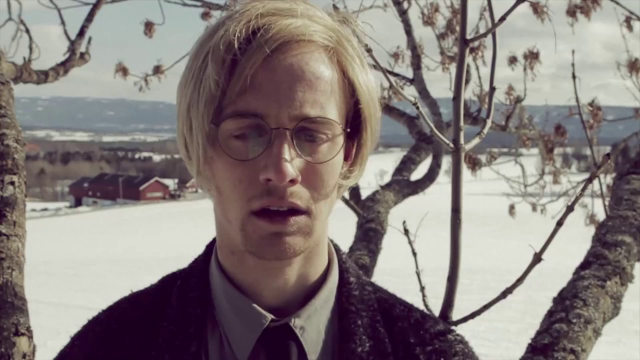
\includegraphics[scale = 0.26]{stuckFrame200}~
		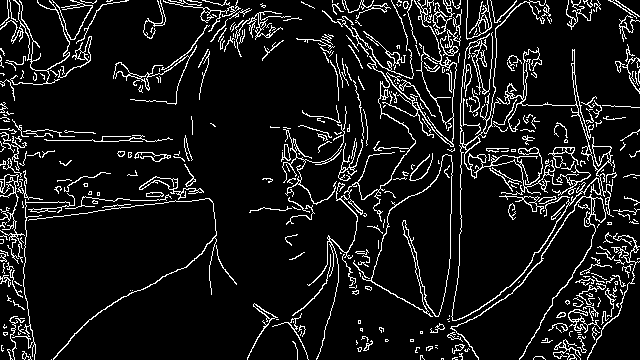
\includegraphics[scale = 0.26]{stuckFrame200D}\newline
		
		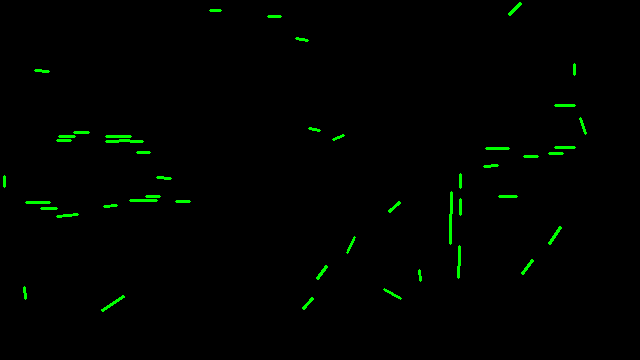
\includegraphics[scale = 0.26]{stuckFrame200L}~
		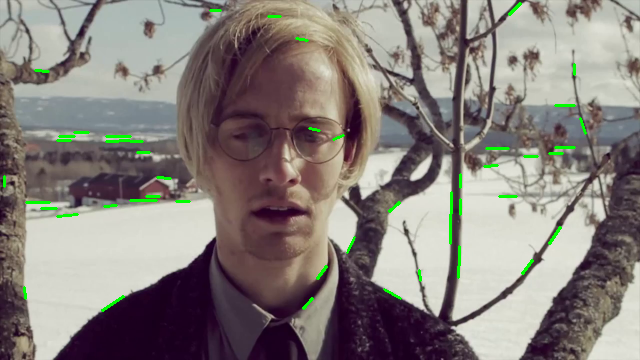
\includegraphics[scale = 0.26]{stuckFrame200O}~
		
	\end{frame}
	
\end{document}